% 请确保文件编码为utf-8,使用XeLaTex进行编译,或者通过overleaf进行编译

\documentclass[answers]{exam}  % 使用此行带有作答模块
% \documentclass{exam} % 使用此行只显示题目

\usepackage{xeCJK}
\usepackage{zhnumber}
\usepackage{graphicx}
\usepackage{hyperref}
\usepackage{amsmath}
\usepackage{booktabs}
\usepackage{enumerate}
\usepackage{amssymb}

\pagestyle{headandfoot}
\firstpageheadrule
\firstpageheader{南京大学}{高级机器学习}{习题集二}
\runningheader{南京大学}
{高级机器学习}
{习题集二}
\runningheadrule
\firstpagefooter{}{第\thepage\ 页(共\numpages 页)}{}
\runningfooter{}{第\thepage\ 页(共\numpages 页)}{}

% no box for solutions
% \unframedsolutions

\setlength\linefillheight{.5in}

% \renewcommand{\solutiontitle}{\noindent\textbf{答:}}
\renewcommand{\solutiontitle}{\noindent\textbf{解:}\par\noindent}

\renewcommand{\thequestion}{\zhnum{question}}
\renewcommand{\questionlabel}{\thequestion .}
\renewcommand{\thepartno}{\arabic{partno}}
\renewcommand{\partlabel}{\thepartno .}


\begin{document}
\Large

\begin{questions}
\question [30] \textbf{半监督学习}

关于半监督学习,课堂上介绍了为什么需要半监督学习以及半监督学习的几种基本做法。在前沿研究中,无论是计算机视觉还是自然语言处理领域,半监督学习仍然是研究重点。下面三个问题分别针对传统半监督学习、深度半监督学习进行拓展介绍。

\begin{parts}
	\part [10] 在TSVM中会对未标记的样本进行标记指派,这个本质上也是一种伪标签的应用。伪标签的含义就是给无标记数据赋予标签,最初这些标签可能绝大多数是错误的,但是会有一些是准确的,将这些准确的筛选出来加入有标记数据训练即可起到扩充训练集的效果。这也是TSVM的主要思想。因此,使用一个预训练模型给未标记数据打标签之后,该怎么做才能尽可能选出那些准确的样本呢?请提供至少三种启发式解决方案并说明理由。(提示:从置信度等角度出发)。试查阅主动学习(Active Learning)相关资料,介绍主动学习并分析其与基于伪标签半监督学习的区别。
	
	\part [10] 标记传播(Label Propagation)是一种非常有效的图半监督学习算法,将样本看做图的顶点,然后将标记从有标记样本扩散到未标记样本。该过程类似于PageRank算法,试描述PageRank算法并比较其与Label Propagation的区别。其余相关的算法还包括:Query Diffusion (QD)等。QD算法先计算样本点之间相似度$a_{ij}=s(x_i,x_j) \geq 0, \forall i, j \in [n]^2$(假设该相似度对称,即$a_{ij}=a_{ji}$),构成亲和矩阵(Affinity Matrix) $A\in \mathcal{R}^{(n+m)\times (n+m)}$,然后对每个样本点计算近邻集合$NN_k(i)$,$k$代表近邻样本数目,记$D=\text{Diag}(\text{sum}(A, 0))$表示亲和矩阵的列和组成的对角阵,那么标准化的亲和矩阵为$S=D^{-1/2}AD^{-1/2}$。记初始的扩散标记为$f_0 \in \mathcal{R}^{n+m}$,例如是前$n$个有标记数据的标记(回归问题的预测值)和以0填充的$m$个未标记数据的标记。那么试着给出其扩散的迭代公式,并分析其意义。
	
	\part [10] 课堂上介绍的传统半监督学习有几种经典假设:聚类假设和流形假设。前者假设数据存在聚簇结构,同一簇的样本属于同一类别;后者假设数据分布在一个流形结构上,邻近的样本有相同的输出值。在深度半监督学习中,有某些其它常用的假设:一致性假设(Consistency Assumption)和低熵(Low Entropy Assumption)假设。一致性假设指的是相似的样本具有相似的输出,低熵假设则是指预测输出结果尽可能具有较低的信息熵。在分类问题中,深度学习常用损失为交叉熵损失。假设有标记样本为$\{(x_i^l, y_i^l)\}_{i=1}^n$,其中$y_i^l \in \{1,2,\cdots,C\}$代表类别,$C$表示类别数目。无标记样本记为$\{x_j^u\}_{j=1}^m$。记神经网络拟合的函数为$f_{\theta}(x)$,$\theta$代表待优化参数。假设该神经网络最后一层没有任何激活函数,即输出是每个类别的打分,打分可正可负,即$f_{\theta}(x) \in \mathcal{R}^C$。请写出交叉熵函数的具体形式(可参考:Softmax + Cross Entropy),以及带有一致性假设和低熵假设优化目标的损失函数(一致性假设中相似的样本可以根据数据增强来获得,即:$\hat{x}_j^u=\text{DataAugmentation}(x_j^u)$)。

\end{parts}

\begin{solution}
	\begin{parts}
		\part 
		(a)三种启发式解决方案:\\
		一、基于聚类:我们分别计算不同类型的有标签样本的中心点,然后依次计算半监督学习预测的未标记样本与各个类中心点之间的距离,
		从中选取类别一致并且距离较小的部分视为分类正确的样本。\\
		二、计算样本的可信度:使用有标记样本训练模型得到划分超平面,计算各个未标记样本到超平面的距离,距离越近代表该样本的不确定性越大,分类可信度越低。\\
		三、间隔法:对于一对未标记样本$x^u_i,x^u_j$,若预训练模型给出的标记$y^u_i,y^u_j$不同,
		同时对应的松弛变量$\zeta_i+\zeta_j>2$,这意味着这对样本被分配的标签很有可能不正确。\\
		~\\
		(b)介绍主动学习并分析与...的区别:\\
		主动学习也是半监督学习的一种,其主要思路在于,对于部分较“难”分类的样本,由人工进行
		标注后利用新的数据进行训练,从而提升模型的性能。\\
		~\\
		区别:基于伪标签的半监督学习每次迭代都会选取一部分高置信度的伪标签样本加入原有的有标记数据集,得到
		新的数据集后再进行下一轮训练,并不需要人力的参与。\\
		而主动学习则是直接选出分类不准确的样本交由人工进行标记,使用了专家知识。

		\part 
		(a)描述PageRank并与Label Propagation比较区别:\\
		PageRank算法是在有向图上定义一个一阶马尔可夫链,描述随机游走者沿着有向图随机访问各个结点的行为。在一定条件下,极限情况访问每个结点的概率收敛到平稳分布,
		这时各个结点的平稳概率值就是其PageRank值,表示结点的重要度,该数值越高表明该结点被访问的概率越大。通常我们用如下公式迭代地计算PR值直到误差小于阈值或者
		达到迭代次数
		$$PR(p_i)=\alpha\sum\limits_{p_j\in M_{p_i}}\frac{PR(p_j)}{L(p_j)}+\frac{1-\alpha}{N}$$
		其中,$M_{p_i}$代表指向$p_i$的节点集合,$L(p_j)$是节点$p_j$的出度,$N$是节点数目,$\alpha$是阻尼因子,常取值为0.85\\
		~\\
		二者的区别:\\
		(1)PageRank可以看作是随机游走,但LPA并非如此\\
		(2)在迭代时,对于概率转移矩阵PageRank是进行行乘,LPA是进行列乘,而概率转移矩阵
		只保证行和为1(列和未必是1),这导致PageRank在每轮迭代中保证了所有节点的权重总和为1,LPA的迭代结果是每个节点自身的类型分布是一个概率分布。\\
		(3)PageRank是无监督学习算法,而Label Propagation的节点有标签,是半监督学习。\\
		(4)标签传播算法是基于聚类假设的,即假定数据存在簇结构,同一个簇的样本属于同一个类
		别,因而其最终的label 是根据相似数据得到的。\\
		~\\
		(b)扩散的迭代公式:$$f_{t+1}=\alpha Sf_t+(1-\alpha)y$$\\
		这代表着,在随机游走模型中,我们有$\alpha$的概率按照亲和矩阵给出的概率进行转移,
		还有$1-\alpha$的概率随机转移到某个节点。
		\part 交叉熵函数为
		$$L=-\frac{1}{n}\sum\limits_{k=1}^n\sum\limits_{j=1}^C\mathbb{I}(y^l_k=j)logp^l_{kj}-\frac{1}{m}\sum\limits_{k=1}^m\sum\limits_{j=1}^Cp_{kj}logp_{kj}$$
		其中,$p_{kj}^l=\frac{expf_{\theta}(x_k^l)_j}{\sum\limits_{i=1}^Cexp(f_{\theta}(x_k^l)_i)},p_{kj}=\frac{expf_{\theta}(x_k^u)_j}{\sum\limits_{i=1}^Cexp(f_{\theta}(x_k^u)_i)}$\\
		加入一致性假设和低熵假设后,我们的优化目标为$$\min \alpha_lL_1+\alpha_uL_2$$
		其中,$L_1$是$L$的第一项,$L_2$是$L$的第二项。
	\end{parts}
\end{solution}


\question [30] \textbf{概率图模型基础}

	本题考查概率图模型中的隐马尔科夫模型和条件随机场相关内容。
	\begin{parts}
		\part [10] 概率图模型是一类用图来表达变量相关关系的概率模型,其中,隐马尔可夫模型(Hidden Markov Model, HMM)和条件随机场(Conditional Random Field, CRF)皆用于解决序列标注任务。请对比两种模型的区别。
		
		\part [10] 条件随机场与对数几率回归(Logistic Regression)都可看作是对数线性模型(Log-linear model)的特例,假设$x$是样本点,$y$是标签,对数线性模型可写成如下的形式:
		\begin{equation}
			p(y \mid x ; w)=\frac{\exp \sum_{j} w_{j} F_{j}(x, y)}{\sum_{y^{\prime}} \exp \sum_{j} w_{j} F_{j}\left(x, y^{\prime}\right)}
		\end{equation}
		其中,$F_j$表示第$j$个特征函数,$w_j$为对应的权重,分母部分为归一化项。请根据以上公式说明条件随机场和对数几率回归的差异。
		
		\part [10] 在HMM的使用过程中会发现以下两个缺点:一、对于每个状态,HMM模型只能捕捉到该状态对应观测的依赖关系,拿文本翻译任务来说,是需要考虑周围单词的信息,甚至是整段文本的信息;二、并且目标函数和预测目标函数并非匹配,具体指的是HMM学习了状态和观测的联合分布$P(\mathbf{Y}, \mathbf{X})$,但在预测时使用的是条件概率$P(\mathbf{Y} \mid \mathbf{X})$. (a)具体说明最大熵马尔可夫模型(Maximum Entropy Markov Model, MEMM)如何解决以上两点,是否还有其他方法呢?(b) MEMM中出现了新的问题:标签偏移问题(label bias problem),请说明为什么会出现该问题,并思考如何解决。参考文献:  Maximum entropy Markov models for information extraction and segmentation.
	\end{parts}
	
	\begin{solution}
		\begin{parts}
			\part 
			(1)、条件随机场是无向图模型,隐马尔可夫模型是有向图模型\\
			(2)、条件随机场是判别式模型,隐马尔可夫是生成式模型\\
			(3)、CRF可以取不同的特征函数和权重来进行优化,并且在某种选择下就等价于HMM\\
			(4)、HMM是对转移概率和表现概率直接建模,很依赖初始值的设定,且容易陷入局部最优;
			但是CRF则是在全局上建立统一的概率模型,得到的是全局最优解。\\
			(5)、HMM假设观测节点之间是独立的,而CRF没有HMM严格
			的独立性假设条件。\\
			\part 
			记特征函数为$f$\\
			条件随机场的概率计算可以写成
			$$P(y|x)=\frac{exp(\sum_{j=1}^m\sum_{i=1}^n\lambda_jf_j(x,i,y_i,y_{i-1}))}{\sum_{y'}exp(\sum_{j=1}^m\sum_{i=1}^n\lambda_jf_j(x,i,y^{'}_i,y^{'}_{i-1}))}$$
			~\\
			对数几率回归的概率计算如下式:
			$$p(y|x)=\frac{exp\sum_{j=1}^N w_{j} f_{j}(x, y)}{\sum_{y^{\prime}} \exp \sum_{j=1}^N w_{j} f_{j}\left(x, y^{\prime}\right)}$$
			~\\
			差异:\\
			(1)、逻辑回归是用于分类的对数线性模型,CRF是标签序列的对数线性模型。\\
			(2)、LR可以看作是CRF的一种特殊情况。\\
			(3)、这二者在特征函数的选择上有所区别,CRF选取的是针对序列的,而对数几率回归中则针对二元特征。\\
			\part 
			(a)、\\
			对于第一点,MEMM考虑了相邻状态之间的依赖关系,且考虑整个观察序
			列,通过$P(s_t|s_{t-1},o_t)$,我们可以建立全局上的依赖关系。\\
			~\\
			对于第二点,MEMM模型计算$P(s_{t}|s_{t-1},o_t)$时利用到了当前观测值和前一个状态,这使得
			整个序列的概率表达式$P(Y|X)=P(y_1,y_2,...,y_n)=P(y_1|x)P(y_2|y_1,x)...P(y_n|y_{n-1},x)$
			即MEMM计算的目标就是P(Y|X),这也就解决了HMM的第二个缺点。\\
			\\
			(b)、MEMM所做的是局部归一化,每个状态都有一个概率模型,在每个状态转移时都要进行归一化。如果某个状态只有一个后续 状态,那么该状态到后续状态的跳转概率即为1。
			这样,不管输入为任何内容,它都向该后续状态跳转。\\
			~\\
			为了解决该问题,可以参照全局归一化的CRF算法,该算法在所有的状态上建立了一个统一的概率模型,
			此时在进行归一化过程中,即使某个状态只有一个后续状态,它到该后续状态的跳转概率也不会为1,
			从而避免了label bias的问题。\\
			具体操作上,我们将MEMM的概率表达式中的分母进行修改,使用CRF中的归一化方式即可。\\
			令$A_{ij}$为概率转移矩阵\\
			记$f(\boldsymbol{y};x)=f(y_1;x)+\sum\limits_{k=2}^n(A_{k-1,k}+f(y_k;x))$\\
			CRF的概率分布可以写成$$p(\boldsymbol{y}|x)=\frac{exp(f(y_1,...,y_n,;x))}{\sum\limits_{y_1,...,y_n}exp(f(y_1,...,y_n;x))}$$
			而MEMM导出的概率分布如下式:$$p(\boldsymbol{y}|x)=\frac{exp(f(y_1,...,y_n;x))}{(\sum\limits_{y_1}e^{f(y_1;x)})(\sum\limits_{y_2}e^{A_{12}+f(y_2;x)})...(\sum\limits_{y_n}e^{A_{n-1,n}+f(y_n;x)})}$$
			有概率分布表达式可见,MEMM是局部归一化的,CRF是全局归一化的,故而只要将MEMM中的分母换成CRF中的,即可避免label bias的问题。
		\end{parts}
	\end{solution}
	
\question [40] \textbf{概率图模型进阶}

	本题研究概率图模型里面的变分推断技术。现定义联合分布如下:
	$$p(\mathbf{t}, \boldsymbol{w}, \alpha)=p(\mathbf{t} \mid \boldsymbol{w}) p(\boldsymbol{w} \mid \alpha) p(\alpha)$$
	其中各具体分布为:
	$$p(\mathbf{t} \mid \boldsymbol{w})=\prod_{n=1}^{N} \mathcal{N}\left(t_{n} \mid \boldsymbol{w}^{T} \boldsymbol{\phi}_{n}, \beta^{-1}\right)$$
	$$p(\boldsymbol{w} \mid \alpha)=\mathcal{N}\left(\boldsymbol{w} \mid \mathbf{0}, \alpha^{-1} \boldsymbol{I}\right)$$
	$$p(\alpha)=\operatorname{Gam}\left(\alpha \mid a_{0}, b_{0}\right)=\frac{{b_0}^{a_0} \alpha^{a_0-1} e^{-b_0 \alpha}}{\Gamma(a_0)}$$
	这里,$\mathcal{N}$代表高斯分布,$\operatorname{Gam}\left(\alpha \mid a_{0}, b_{0}\right)$表示变量为$\alpha$,参数为$a_0,b_0$的Gamma分布。
	\begin{parts}
		\part [10] 请使用盘式记法表示联合分布$p(\mathbf{t}, \boldsymbol{w}, \alpha)$。
		
		\part [20] 现在需要寻找对后验概率分布$p(\boldsymbol{w}, \alpha \mid \mathbf{t})$的一个近似。使用变分框架进行分解,得到变分后验概率分布的分解表达式为$q(\boldsymbol{w},\alpha) = q(\boldsymbol{w})q(\alpha)$。首先计算$q^*(\alpha)$,考虑$\alpha$上的概率分布,利用教材公式(14.39),只保留与$\alpha$有函数依赖关系的项,试证明
		$$\ln q^*(\alpha)=\left(a_{0}-1\right) \ln \alpha-b_{0} \alpha+\frac{M}{2} \ln \alpha-\frac{\alpha}{2} \mathbb{E}\left[\boldsymbol{w}^{T} \boldsymbol{w}\right]+\text { 常数 }$$
		这里$M$表示与$\boldsymbol{w}$和$\alpha$无关的常数。
		
		\part [10] 由上一题得到的结果,观察发现这是Gamma分布的对数,因此$q^*(\alpha)$仍然服从如下Gamma分布
		$$q^{*}(\alpha)=\operatorname{Gam}\left(\alpha \mid a_{N}, b_{N}\right)$$
		问:(a)计算$a_{N}, b_{N}$的具体值(提示:由上一题计算Gamma分布对数$\ln p(\alpha)$的结果观察$\alpha$和$\ln\alpha$的系数便可简单解决)
		(b)比较$q^{*}(\alpha)$与$p(\alpha)$的相似度,总结变分推断的效果。(简单作答即可)
	\end{parts}
	
\begin{figure}[h]
	\centering
	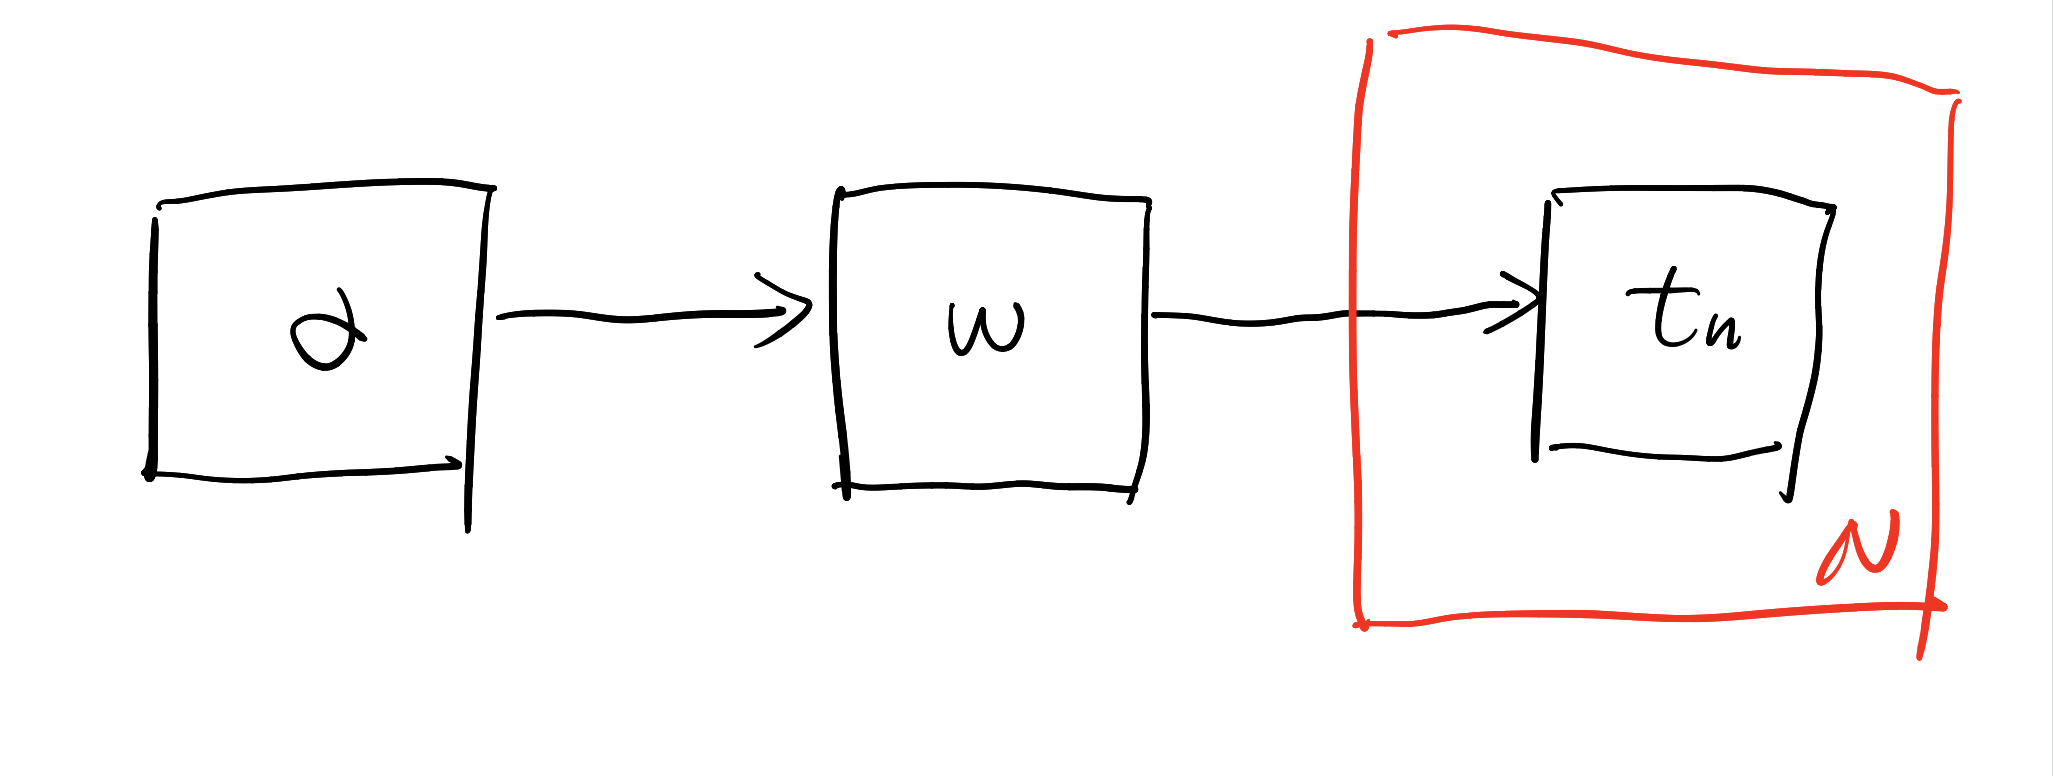
\includegraphics[width=18cm,height=8cm]{p3.png}
	\caption{盘式记法图片}	
\end{figure}	
	
	\begin{solution}
		\begin{parts}
			\part 如图所示
			\part 
			由教材公式
\begin{align*}
	lnq^*(\alpha)&=E_{\boldsymbol{w}}[lnp(\alpha,\boldsymbol{w},t)]+C\\
	&=E_{\boldsymbol{w}}[lnp(t|\boldsymbol{w})p(\boldsymbol{w}|\alpha)p(\alpha)]+C\\
	&=E_{\boldsymbol{w}}[lnp(t|\boldsymbol{w})]+E_{\boldsymbol{w}}[lnp(\boldsymbol{w}|\alpha)]+E_{\boldsymbol{w}}[lnp(\alpha)]+C\\
	&=lnp(\alpha)+E_{\boldsymbol{w}}[\sum\limits_{n=1}^N\mathcal{N}(t_n|\boldsymbol{w}^T\phi_n,\beta^{-1})]+E_{\boldsymbol{w}}[ln\mathcal{N}(\boldsymbol{w}|\mathbf{0},\alpha^{-1}\boldsymbol{I})]+C\\
\end{align*}
由于只保留与$\alpha$有关的项,故忽略上式中的第2项,有:\\
\begin{align*}
	lnq^*(\alpha)&=lnp(\alpha)+E_{\boldsymbol{w}}[ln\mathcal{N}(\boldsymbol{w}|\mathbf{0},\alpha^{-1}\boldsymbol{I})]+C\\
	&=a_0lnb_0+(a_0-1)ln\alpha-b_0\alpha-ln\Gamma(a_0)+E_{\boldsymbol{w}}[ln\mathcal{N}(\boldsymbol{w}|\mathbf{0},\alpha^{-1}\boldsymbol{I})]+C\\
	&=(a_0-1)ln\alpha-b_0\alpha+E_{\boldsymbol{w}}[ln\mathcal{N}(\boldsymbol{w}|\mathbf{0},\alpha^{-1}\boldsymbol{I})]+C_1\ \ (a)
\end{align*}
现在计算$E_{\boldsymbol{w}}[ln\mathcal{N}(\boldsymbol{w}|\mathbf{0},\alpha^{-1}\boldsymbol{I})]$\\
	
\begin{align*}
	E_{\boldsymbol{w}}[ln\mathcal{N}(\boldsymbol{w}|\mathbf{0},\alpha^{-1}\boldsymbol{I})]
	&=E_{\boldsymbol{w}}[-\frac{1}{2}\boldsymbol{w}^T(\alpha^{-1}\boldsymbol{I})\boldsymbol{w}-ln(2\pi)^{\frac{D}{2}}\cdot|\alpha^{-1}\boldsymbol{I}|^{\frac{1}{2}}]\\
	&=-\frac{\alpha}{2}\mathbb{E}[\boldsymbol{w}^T\boldsymbol{w}]-\frac{1}{2}(Dln2\pi+ln|\alpha^{-1}\boldsymbol{I}|)\\
	&=-\frac{\alpha}{2}\mathbb{E}[\boldsymbol{w}^T\boldsymbol{w}]+\frac{M}{2}ln\alpha+C_2
\end{align*}
上式中,$D$是$\boldsymbol{w}$的维数,$M$是$\boldsymbol{I}$的维度,与$\alpha,\boldsymbol{w}$都无关,将结果带入$(a)$式,得到
$$lnq^*(\alpha)=(a_0-1)ln\alpha-b_0\alpha+\frac{M}{2}ln\alpha-\frac{\alpha}{2}\mathbb{E}[\boldsymbol{w}^T\boldsymbol{w}]+C_1+C_2$$
$C_1,C_2$均为常数,证毕

	\part
	(a)$q^*(\alpha)=\frac{b_N^{a_N}\alpha^{a_N-1}e^{-b_N\alpha}}{\Gamma(a_N)}$\\
	故$lnq^*(\alpha)=(a_N-1)ln\alpha-b_N\alpha+a_Nlnb_N-ln\Gamma(a_N)$\\
	与2中对比系数可以求得$a_N=a_0+\frac{M}{2},b_N=b_0+\frac{1}{2}\mathbb{E}[\boldsymbol{w}^T\boldsymbol{w}]$\\
	~\\
	(b)相似度可以用差异度来考量,故计算$KL(q^*||p)$\\
\begin{align*}
	KL(q^*||p)&=\int_{-\infty}^{\infty}q^*(\alpha)ln\frac{q^*(\alpha)}{p(\alpha)}d\alpha\\
	&=\int_{-\infty}^{\infty}q^*(\alpha)[\frac{M}{2}ln\alpha-\frac{\alpha}{2}\mathbb{E}[\boldsymbol{w}^T\boldsymbol{w}]+C]d\alpha
\end{align*}
	注意到右半部分的乘积项是$lnq^*(\alpha)$的一部分,故积分项$<q^*(\alpha)lnq^*(\alpha)<[q^*(\alpha)]^2$,
	故而$KL$散度值较为接近于0,即$q^*,p$差异很小。\\
	直观上也较易理解,二者均为Gamma分布,仅在参数上有着较小差别,即
	$$
    \begin{cases}
        a_N=a_0+\frac{M}{2} \\
        b_N=b_0+\frac{1}{2}\mathbb{E}[\boldsymbol{w}^T\boldsymbol{w}]  
    \end{cases}
$$

	\end{parts}
	\end{solution}
	
\end{questions}


\end{document}